\documentclass{article}
\usepackage[spanish]{babel}
\usepackage[utf8]{inputenc}
\usepackage{mathtools}
\usepackage{graphicx}
\usepackage[usenames]{color}


\title{\Huge Aplicaciones de guía para personas con discapacidad visual}

\begin{document}
	
	\begin{titlepage}
		\maketitle
		\thispagestyle{empty}
	\end{titlepage}
	
	%ABSTRACT
	\begin{abstract}
	    En los últimos años ha aumentado la concienciación acerca de la importancia de desarrollar tecnologías accesibles e inclusivas, de modo que, concretamente, cada vez son más las aplicaciones que tratan de reducir las limitaciones que antes las convertían en inalcanzables para personas con discapacidad visual.
	    \\
	    A continuación haremos un pequeño estudio sobre qué apliaciones de accesibilidad ya existen en el campo de la navegación, bien sea por interiores o exteriores, y cómo funcionan.
	
	\end{abstract}
	
	%PRIMERA APP
	\section{Google Maps}
		El pasado 10 de Octubre de 2019, en el World Sight Day, Google dió a conocer la última actualización de la famosa aplicación "Google Maps". Esta incluiría una nueva característica desarrollada desde cero por y para personas con discapacidad visual que convertiría a la misma en una app accesible.
		\\
		\\
		El proyecto consiste en la implementación de una nueva funcionalidad, que facilita la posibilidad de recibir instrucciones de voz más detalladas y nuevos tipos de anuncios verbales muy útiles para las rutas de a pie.
		\\
		Algunas de las nuevas instrucciones incluídas son: informar de manera proactiva que estás en la ruta correcta, la distancia hasta el próximo giro, la dirección en la que estás caminando, avisos para cruzar con precaución si te aproximas a una gran intersección, notificaciones en caso de ser redirigido por causa de haber abandonado accidentalmente la ruta correcta, etc. De esta manera, la aplicación pretende brindar de independencia a las personas que padecen ceguera tratando de que se sientan cómodas y seguras a la hora de explorar lugares nuevos y desconocidos.
		\\
		\\
		La guía de voz detallada para la navegación está actualmente en desarrollo, estando ya disponible en inglés en los Estados Unidos y en japonés en Japón. Su soporte para otros idiomas y países sigue en camino.
		\\
		\\
		\textcolor{blue}{Link: https://blog.google/products/maps/better-maps-for-people-with-vision-impairments/}
		\\
		\\
		En cuanto al desplazamiento por interiores, Google Maps ha incluido mapas de interiores. Entre los edificios que tienen esta funcionalidad destacan los aeropuertos, centros, comerciales, estadios y los lugares con transporte público. 
		\\
		A continuación vemos un ejemplo del famoso Madison Square Garden de Nueva York: 
		
		 \begin{figure}[h!]
			\centering
			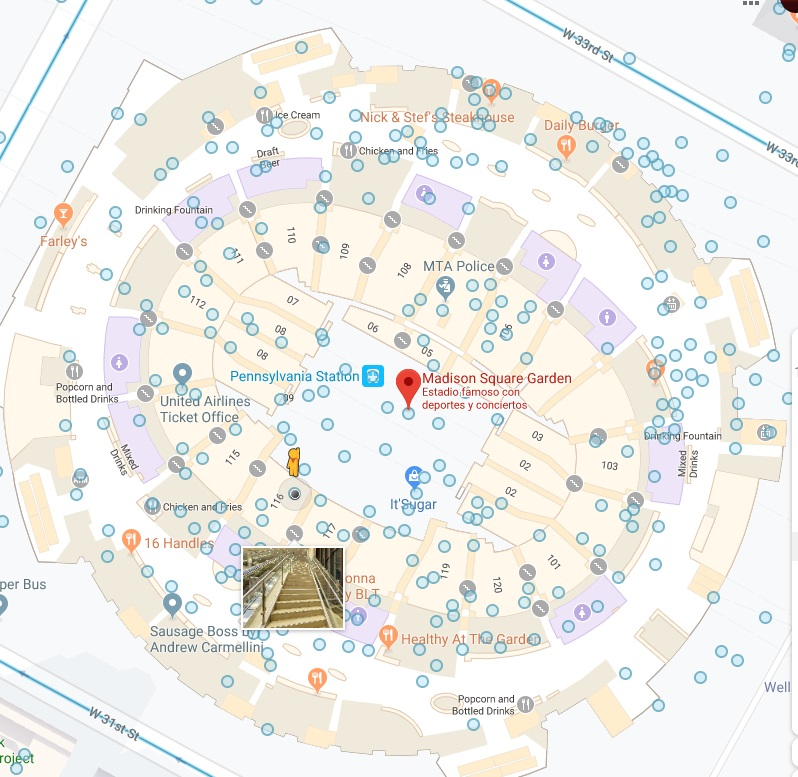
\includegraphics[width=0.6\textwidth]{MadSq2}
			\caption{Basta con ampliar para que Maps nos muestre el mapa del edificio. Arrastrando el muñequito de Google Street View podemos posicionarnos en el interior.}
			\label{fig:ejemplo}
		\end{figure}
		
		 \begin{figure}[h!]
			\centering
			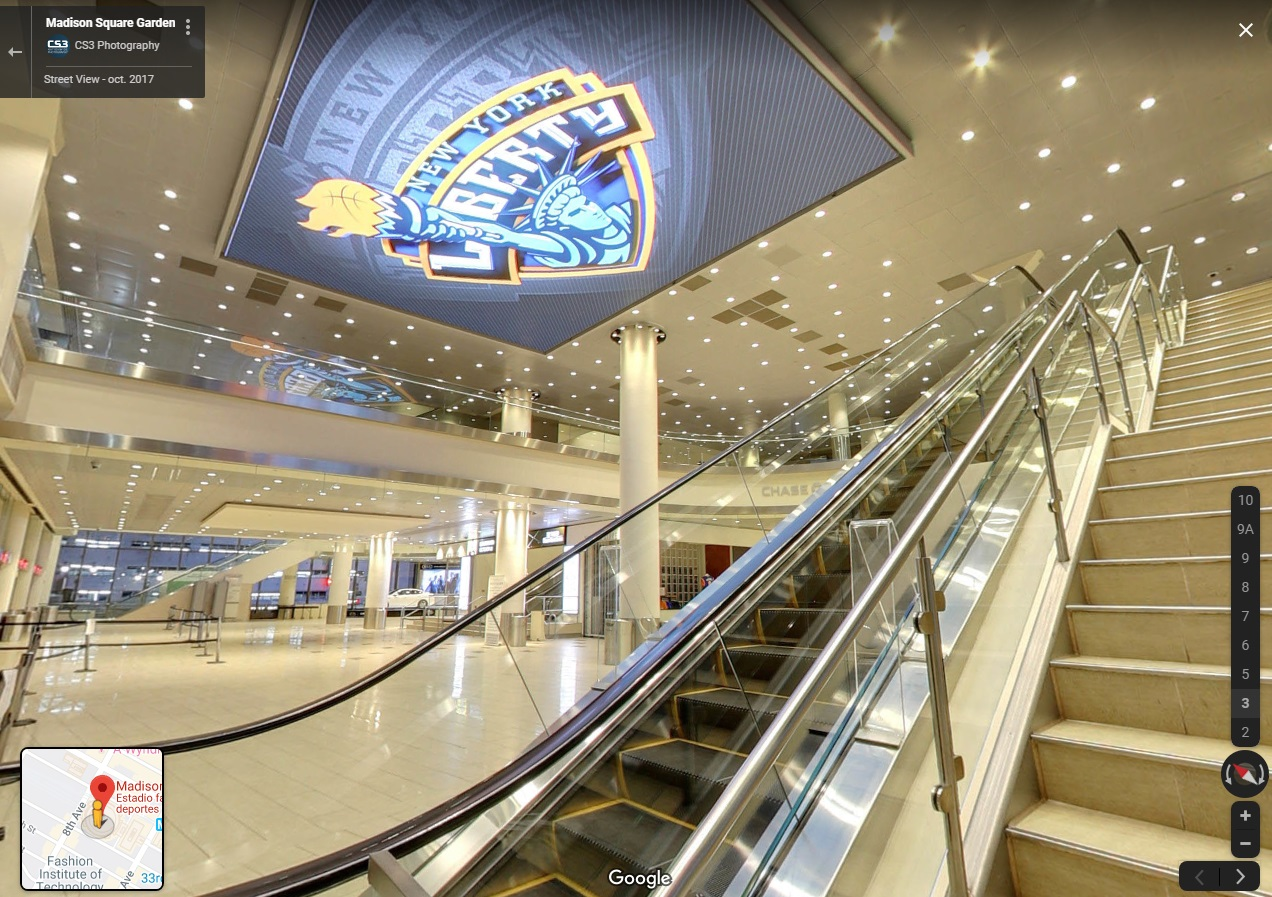
\includegraphics[width=0.6\textwidth]{MadSq3}
			\caption{Vista del interior del Madison Square Garden. }
			\label{fig:ejemplo}
		\end{figure}
	
		Desde la vista del interior puedes desplazarte por todo el edificio de la misma manera que lo haríamos con el Street View convencional aunque, no tenemos la posibilidad de buscar por información extra. Por ejemplo, localizar dónde están los baños del edificio.
		\\
		\\
		\textcolor{blue}{Link: https://www.google.es/intl/es/maps/about/partners/indoormaps/}		
		\\
		Este es un proyecto colaborativo, desde la web nos permiten actualizar planos. Además, está disponible tanto para ordenador como plataformas Android e iOS. 
	
		
	%SEGUNDA APP
	\section{BlindSquare}
	Es una de las aplicaciones guía más usadas, se usa en más de 130 y está disponible en 25 idiomas, entre ellos el español. Esta aplicación, desarrollada para iOs y diseñada para personas con discapacidad visual, proporciona una guía tanto en exteriores como en interiores. Además, describe el entorno y anuncia puntos de interés para el usuario (como pueden ser lugares muy populares o visitados frecuentemente). Lo más importante es que permite interactuar mediante voz, gracias al controlador de música de Apple. 
	\\
	\\
	BlindSquare determina tu posición mediante localización GPS y, a partir de ahí, puede darte información sobre las proximidades desde Foursquare y OpenStreetMap. Como restaurantes a 200m, por ejemplo. Además de ofrecer una guía completa de origen a destino.
	\\
	Cuenta con algunos atajos como sacudir el móvil para que nos diga la ubicación actual. También se pueden establecer filtros, si solo queremos recibir información sobre restaurantes podemos filtrar el resto de notificaciones como estaciones de tren o librerías.
	\\
	\\
	Para la localización por interiores, esta aplicación utiliza iBeacons para solventar el problema de posicionamiento. Por ejemplo, si que quieren buscar los ascensores de un centro comercial y este centro está provisto con iBeacons, la aplicación nos guiará hasta llegar a ellos.
	\\
	\\
	Puntos fuertes de esta aplicación:
	\begin{itemize}
		\item Da información sobre los metros que quedan hasta llegar a un determinado objetivo. Resulta útil porque si van disminuyendo sabes que vas por el camino adecuado.
		\item Utiliza indicaciones reloj: a las 10, a las 3,...
		\item Se pueden añadir lugares en la lista de lugares personalizados.
		\item Puedes ir girando con el móvil y te va indicando lo que tienes enfrente. 
		\item También tiene opción de simulación, que permite prepararse un camino antes de ir.
		\item (App en uso) Desde google Maps indica "sureste", como no sabes dónde está abres BlindSquare para que te lo indique.
		\item Permite ser más autónomo y descubrir nuevos sitios.
		\item Te da las opciones por adelantado. Si estás en un supermercado te avisa de una escalera mecánica antes de llegar para que decidas si cogerla o no.
		\item Permite llevar las manos libres.
		\item Incluye un lector de códigos QR, es más cómodo porque puede dar más información que la línea braille.
	\end{itemize}

	Lo malo: cuesta 40 libras.
	\\
	\\
	\textcolor{blue}{Link iOS accesibility: 	https://developer.apple.com/accessibility/ios/
	\\
	Otras apps: https://www.henshaws.org.uk/wp-content/uploads/2017/06/24-Apps-eBook-1.pdf
	\\
	BlindSquare: https://www.blindsquare.com
	\\
	Video sobre BlindSquare: https://www.youtube.com/watch?v=ITw1Gs6tHLg
	\\
	Video de uso blindSquare en español y exterior: https://www.youtube.com/watch?v=i-5dosYeXw0
	\\
	Video de uso blindSquare en interiores: https://www.youtube.com/watch?v=9jH-Bdjmgb4
	\\
	Otro: el lector del QR en 5:40
	https://www.youtube.com/watch?v=AZUphzNVf48
	}
	
	
\end{document}
© 2019 GitHub, Inc.
Terms
Privacy
Security
Status
Help
Contact GitHub
Pricing
API
Training
Blog
About

